% Drawing 122/01-2 -- folder 122, batch 01, archive page 4 (PDF page 5).
% Transcription: à gauche et à droite, deux croquis de flèches entre $\partial P$, $\widetilde{\partial P}$, $\partial P'$, $\widetilde{\partial P} - \partial P$, $\widetilde{\partial P} - \partial P'$ et $P - P' = \widetilde{\partial P} - \partial P'$, avec la mention « équivalences d'\ill{} »
% Kind: two arrow sketches between boundaries of P and P'. Method 2 (schematic redraw from the facsimile). Status: ok.
% Notes: Left: del P' and del P above and below, joined by arrows to tilde-del P - del P and tilde-del P - del P' (each followed by an equivalence sign) and to tilde-del P, with "= P - P'" beside; right: del P -> tilde-del P <- del P', with tilde-del P - del P below and P - P' = tilde-del P - del P' above, and "équivalences d'..." under it (the last word illegible, as in the transcription). Arrow directions as on the page; the left sketch is crossed by the large frame line of the page, not drawn.
% Coordinates: 1 unit = 1 mm = 1/100 of the crop width (bbox in page fractions: [0.05, 0.18, 0.96, 0.36]).
% Redrawn by Claude (claude-opus-5-5), issue #73, 2026-11-07; not checked by a human; not compiled (no TeX in the session).
% Rights: reproduces part of the work -- behind RENDER_TRANSCRIPTS, never published by itself.
\documentclass[tikz,border=3pt]{standalone}
\usepackage{amsmath,amssymb}
\usetikzlibrary{patterns,arrows.meta}
\tikzset{pencil/.style={black!45}, struck/.style={black!35}, mark/.style={circle,draw,inner sep=1.3pt}, pt/.style={circle,fill,inner sep=0.9pt}, opt/.style={circle,draw,fill=white,inner sep=1.1pt}}
\begin{document}
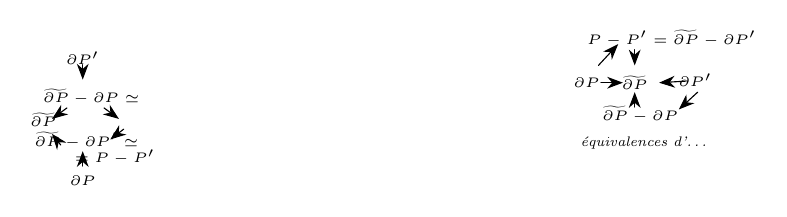
\begin{tikzpicture}[x=1mm,y=1mm,line cap=round,line join=round,font=\scriptsize]
\node[inner sep=1pt] at (15.7,-8) {\tiny $\partial P'$};
\draw[-{Stealth[length=2mm]}] (15.7,-8.8) -- (15.7,-10.7);
\node[inner sep=1pt] at (16.8,-12.9) {\tiny $\widetilde{\partial P}-\partial P\simeq$};
\draw[-{Stealth[length=2mm]}] (13.7,-14.3) -- (11.8,-15.7);
\node[inner sep=1pt] at (10.7,-15.8) {\tiny $\widetilde{\partial P}$};
\draw[-{Stealth[length=2mm]}] (18.4,-14.3) -- (20.3,-15.7);
\node[inner sep=1pt] at (16.2,-18.4) {\tiny $\widetilde{\partial P}-\partial P'\simeq$};
\draw[-{Stealth[length=2mm]}] (12.9,-19) -- (11.8,-17.6);
\draw[-{Stealth[length=2mm]}] (20.9,-17) -- (19.2,-18.3);
\draw[-{Stealth[length=2mm]}] (15.7,-21.7) -- (15.7,-19.8);
\node[inner sep=1pt] at (15.7,-23.6) {\tiny $\partial P$};
\node[inner sep=1pt] at (19.8,-20.6) {\tiny $=P-P'$};
\node[inner sep=1pt] at (90.5,-5.5) {\tiny $P-P'=\widetilde{\partial P}-\partial P'$};
\draw[-{Stealth[length=2mm]}] (85.8,-6.9) -- (85.8,-8.9);
\node[inner sep=1pt] at (85.8,-11.1) {\tiny $\widetilde{\partial P}$};
\node[inner sep=1pt] at (79.7,-11.1) {\tiny $\partial P$};
\draw[-{Stealth[length=2mm]}] (81.5,-11.1) -- (84.3,-11.1);
\node[inner sep=1pt] at (93.5,-10.8) {\tiny $\partial P'$};
\draw[-{Stealth[length=2mm]}] (92.3,-10.9) -- (88.9,-11.1);
\draw[-{Stealth[length=2mm]}] (85.8,-14.2) -- (85.8,-12.3);
\node[inner sep=1pt] at (86.5,-15.1) {\tiny $\widetilde{\partial P}-\partial P$};
\draw[-{Stealth[length=2mm]}] (93.8,-12.3) -- (91.4,-14.5);
\draw[-{Stealth[length=2mm]}] (81.2,-8.9) -- (83.7,-6.2);
\node[inner sep=1pt] at (87.1,-18.8) {\tiny \textit{équivalences d'\ldots}};
\end{tikzpicture}
\end{document}
